%
% 6-darstellung.tex -- Darstellungen von Gruppen
%
% (c) 2022 Prof Dr Andreas Müller, OST Ostschweizer Fachhochschule
%
\section{Darstellungen
\label{buch:gruppen:section:darstellung}}
\kopfrechts{Darstellungen}
Für die Gelfand-Transformation wurden beschränkte Homomorphismen
$G\to\mathbb{C}^*$ benötigt.
Da $\mathbb{C}^*$ eine abelsch Gruppe ist, wird ein Homomorphismus
auf $xy$ und $xy$ den gleichen Wert
\[
h(xy) = h(x)h(y) = h(y)h(x) = h(yx)
\]
annehmen.
Wenn die Gruppe $G$ nicht abelsch und $xy\ne yx$ ist, wird der
Unterschied in den Werten von $h$ nicht mehr sichtbar.
Auch die Gelfand-Transformation kann daher nur einen ``kommutative''
Sicht auf die Gruppe $G$ vermitteln.

Diese Schwierigkeit kann überwunden werden, indem als Funktionswerte
von $h$ nicht nur Zahlen zugelassen werden, sondern beliebige
Matrizen.
Man spricht von einer {\em Darstellung} der Gruppe $G$ durch
Matrizen.
Da die Matrizenmultiplikation im Allgemeinen nicht kommutativ
ist, besteht die Möglichkeit, mindestens einen Teil der
Nichtkommutativität der Gruppe $G$ in den Matrizen $h(x)$
wiederzufinden.

%
% 61-definition.tex -- Darstellungen von Gruppen
%
% (c) 2022 Prof Dr Andreas Müller, OST Ostschweizer Fachhochschule
%

%
% Definition
%
\subsection{Definition}
Viele der klassischen Gruppen sind als Mengen von Matrizen definiert.
Man lernt sie meist bereits in einem Einführungskurs zur linearen Algebra
kennen.
Die Verknüpfung der Gruppenelemente ist die Matrixmultiplikation,
das neutrale Element ist die Einheitsmatrix $I$.
Da sie auch invertierbar sein müssen, liegen sie in der 
allgemeinen linearen Gruppe.
Eine solche Gruppe ist daher eine Teilmenge von $\operatorname{GL}_n(\Bbbk)$
für $\Bbbk=\mathbb{R}$ oder $\Bbbk=\mathbb{C}$.

Die Permutationsgruppe $S_n$ von $n$ Elementen operiert durch 
Vertauschungen.
Zu jeder Permutation $\sigma\in S_n$ lässt sich die Matrix $P_\sigma$
mit den Matrixelementen
\[
(P_\sigma)_{ik}
=
\begin{cases}
1&\qquad\text{für $i=\sigma(k)$}\\
0&\qquad\text{sonst}.
\end{cases}
\]
konstruieren.
Man kann sofort nachrechnen, dass $P_{\sigma\pi} = P_\sigma P_\pi$,
dass $P_{e}=I$ und $P_{\sigma^{-1}}=P_\sigma^{-1}$.
Die Menge der Matrizen
$P_n=\{P_\sigma\mid\sigma\in S_n\}\subset\operatorname{GL}_n(\mathbb{R})$
ist eine Gruppe von Matrizen.

Man kann die Relation, dass $S_n$ in Form der Permutationsmatrizen $P_n$
in $\operatorname{GL}_n(\mathbb{R})$ enthalten ist, auch als Homomorphismus
\[
\varrho
\colon 
S_n
\to
\operatorname{GL}(\mathbb{R})
:
\sigma
\mapsto
P_\sigma
\]
verstehen.
Noch etwas allgemeiner definieren wir eine Darstellung einer Gruppe
wie folgt.

\begin{definition}
Sei $G$ eine Gruppe und $V$ ein $\Bbbk$-Vektorraum.
Ein Homomorphismus $\varrho\colon G\to\operatorname{GL}(V)$
heisst {\em Darstellung} der Gruppe $G$ im Vektorraum $V$.
\index{Darstellung}
Sie heisst {\em $n$-dimensional}, wenn $V$ ein $n$-di\-men\-sio\-na\-ler
Vektorraum ist.
Hat $V$ eine Basis aus $n$ Vektoren, können die linearen
Abbildungen $\varrho(x)$ als Matrizen in $M_{n\times n}(\Bbbk)$
geschrieben werden.
\end{definition}

%
% Die reguläre Darstellung
%
\subsubsection{Die reguläre Darstellung}
Sei $G$ eine endliche Gruppe und $h\in G$.
Die Verknüpfung mit $g$ definiert eine Permutation der Gruppenelemente
durch
\[
\pi_h \colon G \to G : g \mapsto hg.
\]
Zum Gruppenelement $h$ gehört daher die Permutationsmatrix
$P_{\pi_h}\in\operatorname{GL}_n(\mathbb{R})$.
Jede endliche Gruppe hat daher mindestens die Darstellung durch die
Matrizen $P_{\pi_h}$.
Sie heisst die {\em reguläre Darstellung}.

Man kann eine Basis dieser Darstellung bilden, indem man die
Einträge in den Spaltenvektoren mit Elementen der Gruppe indiziert.
Sei $v_g$ der Spaltenvektor, der in der $h$-Zeile eine Eins
hat und lauter Nullen in allen anderen Zeilen.
Die Vektoren $v_h$ sind die die Standardbasis eines $|G|$-dimensionalen
Vektorraumes, auf dem die Gruppe $G$ durch
$\pi_{h}v_{g}=v_{hg}$ wirkt, also durch die Permutaionsmatrix $P_h$.

Die Vektoren $v_h$ kann man auch als die Funktionen
\[
v_h
\colon
G\to\mathbb{R}
:
g\mapsto
\begin{cases}
1&\qquad\text{falls $g=h$}\\
0&\qquad\text{sonst}
\end{cases}
\]
betrachten.
Die Menge der Funktionen $G\to\Bbbk$ bezeichnen wir mit $\Bbbk[G]$,
wobei $\Bbbk=\mathbb{R}$ oder $\Bbbk=\mathbb{C}$ ist.
Die Gruppe $G$ operiert auf den Funktion durch die Translation.
Die Funktion $v_{kh}$ ist genau dann $1$, wenn $g=kh$ ist, also wenn $k^{-1}g=h$
ist.
Dasselbe gilt für die Funktion $g\mapsto v_h(k^{-1}h)$, daher definieren wir
die Translation für beliebige Funktionen $f\colon G\mapsto \mathbb{R}$
durch
\[
T_kf\colon G\to\mathbb{R}:g\mapsto f(k^{-1}g).
\]
Diese Definition deckt sich natürlich mit der
Definition~\ref{buch:gruppen:gruppe:def:translation}.
Die Translation ist also eine Darstellung der Gruppe $G$ auf dem
Vektorraum der Funktionen auf der Gruppe.

Für eine topologische Gruppe $G$ ist die Translation $T_g$ eine 
stetige lineare Abbildung auf dem Vektorraum der stetigen Funktionen
$C_{\mathbb{R}}(G)$, ausserdem ist die Abbildung $g\mapsto T_g$ eine
stetige Abbildung von $G$ in den Vektorraum der linearen Operatoren
auf $C_{\mathbb{R}}(G)$.
Für eine Lie-Gruppe ist $g\mapsto T_g$ sogar eine differenzierbare
Abbildung.
Auch diese Darstellungen von $G$ auf entsprechenden Funktionenräumen
heissen die {\em reguläre Darstellung} von $G$.
\index{reguläre Darstellung}%
\index{Darstellung!regulär}%

%
% Die Standarddarstellung einer Matrizengruppe
%
\subsubsection{Die Standarddarstellung einer Matrizengruppe}
Die reguläre Darstellung ist also eine Art ``universelle Darstellung'',
die man immer konstruieren kann, sie ist allerdings auch etwas kompliziert,
da die Dimension des Vektorraums $V$, auf dem die Gruppenelemente in der
Darstellung wirken, so gross ist wie die Kardinalität der Gruppe.
Von besonderem Nutzen sind Darstellungen, die eine kleine Dimension haben.
Die Elemente einer Gruppe $G\subset\operatorname{GL}_n(\mathbb{R})$
von $n\times n$-Matrizen operiert auf offensichtliche Weise auf einem
$n$-dimensionalen Vektorraum $\mathbb{R}^n$.
Die Untergruppen von $\operatorname{GL}_n(\mathbb{R})$, betrachtet
als abstrakte Gruppen, haben also immer eine $n$-dimensionale Darstellung,
die durch die Einbettung $G\to \operatorname{GL}_n(\mathbb{R})$ entsteht.
Sie heisst die {\em Standarddarstellung}.

%
% Die triviale Darstellung
%
\subsubsection{Die triviale Darstellung}
Für eine beliebige Gruppe $G$ ist die konstante Abbildung
\[
\varrho
\colon
G\to \operatorname{GL}_n(\mathbb{R})
:
g\mapsto I_n
\]
ein Homomorphismus und damit eine $n$-dimensionale Darstellung von $G$.
Sie heisst die {\em triviale $n$-dimensionale Darstellung}.
\index{triviale Darstellung}%
\index{Darstellung!trivial}%

%
% Reguläre Darstellung und Faltung
%
\subsubsection{Reguläre Darstellung und Faltung}
Eine Gruppe $G$ operiert auf den Funktionen auf $G$ durch die 
lineare Operation der Translation $T_g$ für $g\in G$.
Sei $G$ eine endliche Gruppe und $f\colon G\mapsto \mathbb{R}$ eine
Funktion auf $G$.
Da die Translation $T_g$ eine lineare Abbildung ist, können wir die 
sie mit den Koeffizienten $f(g)$ linear kombinieren.
Damit lässt sich eine Operation der Funktion $f$ auf den Funktionen
$h\colon G\to\mathbb{R}$ durch
\begin{equation}
T_fh
=
\sum_{g\in G} f(g)\cdot T_gh
\colon
G\to\mathbb{R}
:
x\mapsto
\biggl( \sum_{g\in G} f(g)\cdot T_gh\biggr) (x)
=
\sum_{g\in G} f(g)h(g^{-1}x)
=
(f*h)(x)
\quad\Rightarrow\quad
T_f
=
\int_G f(g)T_g\,dg.
\end{equation}
definieren.
Die Faltung ist also nichts anderes als die Ausdehnung der regulären
Darstellung von einzelnen Gruppenelementen auf den Vektorraum
der Funktionen auf $G$.

Für eine topologische Gruppe $G$ und eine integrierbare Funktion
$f\colon G\to\mathbb{R}$
lässt sich die Konstruktion ebenfalls durchführen.
Statt einer Summe über die Gruppenelemente muss man allerdings das
Haar-Integral mit den Funktionswerten $f(g)$ als Gewichten verwenden.
Die Funktion $f$ operiert somit auf einer Funktion $h\colon G\to\mathbb{R}$
durch 
\[
T_fh\colon
x\mapsto
\biggl(\int_G f(g) T_gh\,dg\biggr)(x)
=
\int_G f(g) h(g^{-1}x)\,dg
=
(f*g)(x).
\]
Dies zeigt, dass das Studium der reguläre Darstellung nichts anderes
ist als die Untersuchung der Gruppenoperation auf der Gruppe mit Hilfe
der Algebrastruktur, die durch die Faltung erzeugt wird.


%
% 62-rechnen.tex -- Rechnen mit Darstellungen
%
% (c) 2022 Prof Dr Andreas Müller, OST Ostschweizer Fachhochschule
%

%
% Rechnen mit Darstellungen
%
\subsection{Rechnen mit Darstellungen
\label{buch:gruppen:darstellungen:subsection:rechnen-mit-darstellungen}}
Mit Darstellungen kann man ``rechnen'' im folgenden Sinn.
Seien
$\varrho_1\colon G\to\operatorname{GL}_{n_1}(\mathbb{R})$
und
$\varrho_2\colon G\to\operatorname{GL}_{n_2}(\mathbb{R})$
Darstellungen der Gruppe $G$.
Dann kann man eine neue, $n_1+n_2$-dimensionale Darstellung konstruieren,
indem man aus den Matrizen $\varrho_1(g)$ und $\varrho_2(g)$ die
Blockmatrix
\begin{equation}
\varrho(g)
=
(\varrho_1\oplus \varrho_2)(g)
=
\left(\raisebox{-1.15cm}{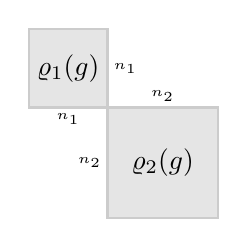
\begin{tikzpicture}[>=latex,thick]
\fill[color=white] (-1.2,-1.2) rectangle (1.2,1.2);
\fill[color=gray!20] (-1.2,1.2) rectangle (-0.2,0.2);
\draw[color=gray!40] (-1.2,1.2) rectangle (-0.2,0.2);
\node at (-0.7,0.25) [below] {\tiny $n_1$};
\node at (-0.25,0.7) [right] {\tiny $n_1$};
\node at (-0.7,0.7) {$\varrho_1(g)\mathstrut$};
\fill[color=gray!20] (-0.2,0.2) rectangle (1.2,-1.2);
\draw[color=gray!40] (-0.2,0.2) rectangle (1.2,-1.2);
\node at (0.5,-0.5) {$\varrho_2(g)\mathstrut$};
\node at (0.5,0.15) [above] {\tiny $n_2$};
\node at (-0.15,-0.5) [left] {\tiny $n_2$};
\end{tikzpicture}}\right).
\label{buch:gruppen:darstellungen:eqn:dirsummatrix}
\end{equation}
Diese Darstellung heisst die {\em direkte Summe} der Darstellungen
$\varrho_1$ und $\varrho_2$.
Für eine natürliche Zahl $k$ soll die
Schreibweise $k\cdot \varrho_1$ als die $k$-fache direkte Summe der
Darstellung $\varrho_1$ interpretiert werden.


%
% 63-vergleich.tex -- Vergleich von Darstellungen 
%
% (c) 2022 Prof Dr Andreas Müller, OST Ostschweizer Fachhochschule
%

%
% Vergleich von Darstellungen
%
\subsection{Vergleich von Darstellungen}
Die Einfachheit der regulären Darstellung hängt davon ab, dass man die
Basis sehr speziell wählen kann.
Eine beliebige Darstellung ist auf den ersten Blick sehr viel weniger gut
durchschaubar, weil eine beliebig gewählte Basis zu Matrizen führt,
die die Natur Gruppe verschleiern können.
Umgekehrt kann auch die reguläre Darstellung verbergen, dass dahinter
eigentlich einfachere Darstellungen stecken, die man besser erkennen
könnte, wenn man eine zweckmässigere Basis verwenden würde.
Das folgende Beispiel illustriert dies.

\begin{beispiel}
\label{buch:gruppen:darstellung:bsp:c3}
Wir betrachten die reguläre Darstellung der zyklischen Gruppe mit
drei Elementen $C_3=\{0,1,2\}$.
Die Gruppenelemente $1,2\in C_1$ werden in der regulären Darstellung
durch die Matrizen
\[
1\mapsto
P_1=
\begin{pmatrix}
0&0&1\\
1&0&0\\
0&1&0
\end{pmatrix}
\qquad\text{und}\qquad
2\mapsto
P_2
=
\begin{pmatrix}
0&1&0\\
0&0&1\\
1&0&0
\end{pmatrix}
=
P_1^2
\]
dargestellt.

Wir verwenden jetzt im Vektorraum $\mathbb{R}^3$, auf dem diese Matrizen
wirken, eine alternative Basis wie folgt:
\[
b_1
=
\frac{1}{\!\sqrt{3}}
\begin{pmatrix}1\\1\\1\end{pmatrix}
,
\qquad
b_2
=
\frac{1}{\!\sqrt{2}}
\begin{pmatrix*}[r]1 \\ -1 \\ 0\end{pmatrix*}
\qquad\text{und}\qquad
b_3
=
\frac{1}{\!\sqrt{6}}
\begin{pmatrix*}[r] 1\\1\\-2\end{pmatrix*}.
\]
Die Basis ist orthonormiert.
Die Wirkung der Matrix $P_1$ auf diesen Basisvektoren ist
\begin{align*}
P_1b_1
&=
b_1\\
P_1b_2
&=
\frac{1}{\!\sqrt{2}}
\begin{pmatrix*}[r]
0\\1\\-1
\end{pmatrix*}
=
(P_1b_2\cdot b_2) b_2
+
(P_1b_2\cdot b_3) b_3
=
-\frac{1}{2}
b_2
+
\frac{\!\sqrt{3}}{2}
b_3
\\
P_1b_3
&=
\frac{1}{\!\sqrt{6}}
\begin{pmatrix*}[r]
-2\\ 1\\1
\end{pmatrix*}
=
(P_1b_3\cdot b_2) b_2
+
(P_1b_3\cdot b_3) b_3
=
-\frac{\!\sqrt{3}}{2}
b_2
-
\frac{1}{2}
b_3
\end{align*}
Die Koeffizienten in der Darstellung der Bildvektoren in der
orthonormierten Basis $\{b_1,b_2,b_3\}$ auf der rechten Seite
können mit Hilfe des Skalarproduktes ermittel werden.
In der Basis $b_i$ bekommt die Matrix $P_1$ also die Matrix
\begin{equation}
\renewcommand{\arraystretch}{1.2}
\tilde{P}_1
=
\begin{pmatrix}
1&0&0\\
0&-\frac12 & \frac{\!\sqrt{3}}2\\
0&-\frac{\!\sqrt{3}}2&-\frac12
\end{pmatrix}
=
\begin{pmatrix}
1&0&0\\
0&\cos\bigl(-\frac{2\pi}{3}\bigr)& -\sin\bigl(-\frac{2\pi}{3}\bigr) \\
0&\sin\bigl(-\frac{2\pi}{3}\bigr)& \phantom{-}\cos\bigl(-\frac{2\pi}{3}\bigr)
\end{pmatrix}.
\label{buch:gruppen:darstellung:bsp:c3:blockform}
\end{equation}
In der neuen Basis zerfällt die Matrix in zwei Blöcke.
Der linke obere Block ist die eindimensionale triviale Darstellung.
der $2\times 2$-Block in der rechten unteren Ecke ist eine Drehmatrix mit
dem Drehwinkel $120^\circ$.

Geometrisch bedeutet die Blockform
\eqref{buch:gruppen:darstellung:bsp:c3:blockform}, dass man den
dreidimensionalen Raum in eine Gerade mit Richtung $b_1$ und
eine dazu senkrechte Ebene mit Basis $\{b_2,b_3\}$ aufteilen
kann.
Auf der geraden operiert die Gruppe $C_3$ trivial, der zweidimensionale
Unterraum ist eine zweidimensionale Darstellung der Gruppe $C_3$.
Es ist also gelungen, die reguläre Darstellung von $C_3$ zu zerlegen
in zwei einfachere Darstellungen.

Die reguläre Darstellung ist die direkte Summe der eindimensionalen
trivialen Darstellung und der zweidimensionalen Darstellung durch
Drehmatrizen.
\end{beispiel}.

Durch Wahl einer geeigneten Basis kann also eine Darstellung umgeformt
werden in eine andere.
Die Basistransformation mit der $n\times n$-Transformationsmatrix
$T:\mathbb{R}^n\to\mathbb{R}^n$ führt die 
Darstellung $\varrho\colon G\to\operatorname{GL}_n(\mathbb{R}$ über
in die Darstellung
\[
\tilde{\varrho}
\colon
G\to\operatorname{GL}_n(\mathbb{R})
:
g\mapsto T\varrho(g)T^{-1}.
\]
Tatsächlich ist $\tilde{\varrho}$ ein Homomorphismus, denn wir können
nachrechnen, dass
\begin{align*}
\tilde{\varrho}(e)
&=
T\varrho(e)T^{-1}
=
TIT^{-1}
=
I
\\
\tilde{\varrho}(gh)
&=
T\varrho(gh)T^{-1}
=
T\varrho(g)\varrho(h)T^{-1}
=
T\varrho(g)T^{-1}T\varrho(h)T^{-1}
=
\tilde{\varrho}(g)
\tilde{\varrho}(h).
\end{align*}

\begin{definition}
Zwei $n$-dimensionale Darstellungen $\varrho_1$ und $\varrho_2$
heissen isomorph, wenn es eine reguläre Matrix $T$ gibt derart, dass
$\varrho_1(g)=T\varrho_2(g)T^{-1}$ für alle $g\in G$.
\end{definition}


%
% 64-schur.tex -- Irreduzible Darstellungen und das Lemma von Schur
%
% (c) 2022 Prof Dr Andreas Müller, OST Ostschweizer Fachhochschule
%

%
% Irreduzible Darstellungen und das Lemma von Schur
%
\subsection{Irreduzible Darstellungen und das Lemma von Schur}
Das Beispiel~\ref{buch:gruppen:darstellung:bsp:c3} hat gezeigt, dass
es möglich ist, die reguläre Darstellung der Gruppe $C_3$ bis auf
Isomorphie in eine direkte Summe zweier einfacherer Darstellungen
zu zerlegen.
Ganz ähnlich wie uns die harmonische Analysis in die Lage versetzt,
Funktionen in Summen von einfacheren Funktionen zu zerlegen, sollte
es auch möglich sein, beliebige Darstellungen in eine Summe von
Bausteinen zu zerlegen.
Dazu muss aber zunächst der Idee der Zerlegbarkeit einer Darstellung
eine eindeutige Definition gegeben werden.

Die Zerlegung der Darstellung von $C_3$ im 
Beispiel~\ref{buch:gruppen:darstellung:bsp:c3} war möglich, weil
der Vektorraum $\mathbb{R}^3$ in zwei Summanden zerlegt werden 
konnte, die unter der Wirkung der Darstellung unverändert sind.
Die Ebene im Beispiel kann aber nicht mehr weiter in eindimensionale
Unterräume aufgespalten werden.

\begin{definition}
\label{buch:gruppen:darstellung:def:irreduzibel}
Eine Darstellung $\varrho\colon G\to \operatorname{GL}_n(\mathbb{R})$ 
heisst {\em irreduzibel}, wenn die einzigen Unterräume, die von allen
Matrizen $\varrho(g)$ in sich abgebildet werden, der Nullraum $\{0\}$
und der ganze Raum $\mathbb{R}^n$ sind.
\end{definition}

Nach dieser Definition ist die reguläre Darstellung von $C_3$ nicht
irreduzibel, da die beiden Unterräume
\[
\mathbb{R}b_1%\begin{pmatrix}1\\1\\1\end{pmatrix}
\qquad\text{und}\qquad
\{
xb_2 + yb_3
\mid
x,y\in\mathbb{R}
\}
\]
beide invariant sind.

\begin{satz}[Lemma von Schur]
\label{buch:gruppen:darstellung:satz:lemmavonschur}
Seien $G$ eine Gruppe sein $\varrho_V\colon G\to \operatorname{GL}(V)$
und $\varrho_W\colon G\to\operatorname{GL}(W)$ irreduzible Darstellungen
von $G$ in den Vektorräumen $V$ und $W$.
Sei ausserdem $f\colon V\to W$ eine lineare Abbildung, die mit den
Darstellungen vertauscht, also
\[
f\circ \varrho_V(g) = \varrho_W(g)\circ f
\]
Dann gilt
\begin{enumerate}
\item $f$ ist entweder die Nullabbildung oder ein Isomorphismus.
\item Falls $V=W$ ist, hat $f$ die Form $f(v)=\lambda v$ mit
$\lambda\in \mathbb{C}$.
\end{enumerate}
\end{satz}

\begin{proof}[Beweis]
Der Kern von $f$ ist der Unterraum
$\operatorname{ker}f = \{v\in V\mid f(v)=0\}$.
Für $v\in\operatorname{ker}f$ ist
$f(\varrho_V(g)v) = \varrho_W(g) f(v) = \varrho_W(g) 0=0$, also ist
$\varrho_V(g)\in\operatorname{ker}f$.
Der Kern von $f$ ist damit ein invarianter Unterraum der Darstellung
$\varrho_V$ von $G$.
Da $\varrho_V$ irreduzibel ist, ist $\operatorname{ker}f$ entweder
der ganze Raum, in diesem Fall ist $f=0$ oder der Kern ist $0$, in diesem
Fall ist $f$ injektiv.

Das Bild von $f$ ist der Unterraum
$\operatorname{im}f = \{f(v)\mid v\in V\}\subset W$.
Dann gilt
$\varrho_W(g)f(v) = f(\varrho_V(g)v)\in\operatorname{im}f$, das Bild von
$f$ ist damit auch ein invarianter Unterraum von $W$.
Da die Darstellung $\varrho_W$  irreduzibel ist, ist $\operatorname{im}f$
entweder der Nullraum, in diesem Fall ist $f=0$, oder das Bild ist der
ganze Raum $W$, in diesem Fall ist $f$ surjektiv.

Die beiden Aussagen zusammen ergeben, dass $f$ entweder die Nullabbildung
ist oder sowohl injektiv wie auch surjektiv ist.
Damit ist 1.~gezeigt.

Bleibt noch 2.~zu zeigen.
Sei $\lambda$ ein Eigenwert der Abbildung $f$ und $v$ ein Eigenvektor.
Dann ist $\lambda I$ eine
Abbildung $V\to V$, die mit der Darstellung vertauscht, denn
\[
\varrho_V(g)\lambda I =
\lambda \varrho_V(g) = \lambda I\varrho_V(g).
\]
Somit ist auch $f-\lambda I$ eine Abbildung $V\to V$, die mit $\varrho_V$
vertauscht.
Nach 1.~muss dies die Nullabbildung oder ein Isomorphismus sein.
Da aber der Eigenvektor $v$ auf $(f-\lambda I)v = \lambda v - \lambda v = 0$
abgebildet wird, kann $f-\lambda I$ nicht ein Isomorphismus sein, somit
ist $f-\lambda I=0$ und damit $f=\lambda I$.
\end{proof}

Die erste Aussage des Lemmas von Schur und sein Beweis zeigen, dass
irreduzible Darstellungen auch nicht teilweise aufeinander abgebildet
werden können.
Wenn eine Abbildung nicht die Nullabbildung ist, dann muss die
ganz Darstellung $V$ ohne Verlust auf die ganze Darstellung $W$
abgebildet werden.
Dies ist nur eine andere Formulierung für die Idee der Irreduzibilität.

Die zweite Aussage des Lemmas von Schur besagt im Wesentlichen, dass
es bis auf Faktor $\lambda$ nur eine Möglichkeit gibt, eine irreduzible
Darstellung mit sich selbst zu vergleichen.


%
% 65-charakter.tex -- Charakter einer Darstellung
%
% (c) 2022 Prof Dr Andreas Müller, OST Ostschweizer Fachhochschule
%

%
% Charakter einer Darstellung
%
\subsection{Charakter einer Darstellung}
Die reguläre Darstellung lässt die Gruppe auf Funktionen auf der
Gruppe operieren.
Der Begriff der irreduziblen Darstellung und das Lemma von Schur
lassen vermuten, dass nur sehr spezielle Funktionen für irreduzible
Darstellungen in Frage kommen.
Es ist daher eine Verbindung zwischen irreduziblen Darstellungen
und Funktionen auf der Gruppe herzustellen.
Diese Funktionen müssen unabhängig sein von der gewählten Basis.

\begin{definition}
\label{buch:gruppen:darstellungen:def:charakter}
Ist $\varrho_V\colon G\to\operatorname{GL}(V)$ eine Darstellung der
Gruppe $G$ im Vektorraum $V$, dann heisst die Funktion
\[
\chi_\varrho
\colon
G
\to
\mathbb{C}
:
g
\mapsto
\tr \varrho_V(g)
\]
der {\em Charakter} der Darstellung $\varrho$.
\end{definition}

Der Charakter einer Darstellung hängt nicht von der Wahl der Basis ab.
Zwei verschiedene Basen im Darstellungsraum $V$ führen auf verschiedene
Matrizen $\varrho_1(g),\varrho_2(g)\in\operatorname{GL}_n(\mathbb{C})$,
die aber durch eine Transformationsmatrix $T$ über die Formel
$\varrho_1(g)=T\varrho_2(g)T^{-1}$ miteinander verbunden sind.
Die Spur dieser Matrizen ist
\[
\tr \varrho_1(g)
=
\tr(T\varrho_2(g)T^{-1})
=
\tr(\varrho_2(g)T^{-1}T)
=
\tr \varrho_2(g),
\]
die Spuren sind also gleich.

Nicht jede Funktion kann ein Charakter sein, wie der folgende Satz
zeigt.

\begin{satz}
\label{buch:gruppen:darstellungen:satz:chareigenschaften}
Sei $\varrho$ eine $n$-dimensionale Darstellung von $G$ dann gilt
\begin{enumerate}
\item $\chi_\varrho(e) = n$
\item $\chi_\varrho(hgh^{-1}) = \chi_\varrho(g)$
\end{enumerate}
\end{satz}

\begin{proof}[Beweis]
Da $\varrho(e)=I_n$ die $n$-dimensionale Einheitsmatrix ist, ist
$\chi_\varrho(e) = \tr \varrho(e) = \tr I_n = n$, was 1.~beweist.
Aussage~3.~folgt aus
$\chi_\varrho(hgh^{-1})
=
\tr (\varrho(h)\varrho(g)\varrho(h)^{-1})
=
\tr \varrho(g)
=
\chi_\varrho(g)
$.
\end{proof}

Der Charakter einer Darstellung ist nur für eindimensionale Darstellungen
ein Homomorphismus, es ist also im Allgemeinen nicht möglich $\chi(g^{-1})$,
aus $\chi(g)$ zu berechnen.
Für endliche Gruppen gibt es aber einen Weg.

\begin{satz}
\label{buch:gruppen:darstellung:satz:charg-1}
Sei $\varrho$ eine $n$-dimensionale Darstellung einer endlichen Gruppe,
dann gilt
$\chi_\varrho(g^{-1}) = \overline{\chi_\varrho(g)}$.
\end{satz}

\begin{proof}[Beweis]
Wir verwenden eine Basis, in der die Matrix $\varrho(g)$ \JN hat.
Die \JN ist eine obere Dreiecksmatrix mit den Eigenwerten
$\lambda_i$ auf der Diagonalen.
Da spätestens die $n$-te Potenz von $g$ das neutrale Element ist und damit
die $n$-te Potenz der Matrix $\varrho(g)$ die Einheitsmatrix ist, müssen
alle Eigenwerte Betrag $1$ haben.
Die inverse Matrix $\varrho(g)^{-1}$ ist ebenfalls eine Dreiecksmatrix
mit den reziproken Eigenwerten $\lambda_i^{-1}$ auf der Diagonalen.
Da die $\lambda_i$ Betrag $1$ haben, ist $\lambda_i^{-1}=\overline{\lambda}_i$
und damit
\[
\chi_\varrho(g^{-1})
=
\tr \varrho(g^{-1})
=
\sum_{i=1}^n \lambda_i^{-1}
=
\sum_{i=1}^n \overline{\lambda}_i
=
\overline{\sum_{i=1}^n \lambda_i}
=
\overline{\tr \varrho(g)}
=
\overline{\chi_\varrho(g)}.
\]
\end{proof}

Der Beweis hängt davon ab, dass die Eigenwerte alle den Betrag $1$ haben,
eine Eigenschaft, die für eine endliche Gruppe dank der \JN leicht zu
erschliessen war.
Wir werden später sehen, dass man in vielen Fällen auch zeigen kann,
dass die Matrizen $\varrho(g)$ alle orthogonal oder unitär sind, was
ebenfalls zur Folge hat, dass die Eigenwerte Betrag $1$ haben.
Schliesslich kann auch die Einschränkung auf beschränkte Funktionen
ebenfalls Eigenwerte mit Betrag verschieden von $1$ ausschliessen.

%
%  Charaktere und Rechenoperationen mit Darstellungen
%
\subsubsection{Charaktere und Rechenoperationen mit Darstellungen}
In Abschnitt~\label{buch:gruppen:darstellungen:subsection:rechnen-mit-darstellungen}
wurden Rechenoperationen mit Darstellungen definiert.
Die direkte Summe $\varrho_1\oplus\varrho_2$ einer $n_1$-dimensionalen
Darstellung $\varrho_1$ und einer $n_2$-dimensionalen Darstellung
$\varrho_2$ ist eine $n_1+n_2$-dimensionale Darstellung.
Die Spur der Matrix~\eqref{buch:gruppen:darstellungen:eqn:dirsummatrix}
ist die Summe der Spuren der Teilmatrizen und daher
\[
\chi_{\varrho_1\oplus\varrho_2}
=
\chi_{\varrho_1}
+
\chi_{\varrho_2}.
\]

Wenn sich eine Darstellung in eine Summe von irreduziblen Darstellungen
zerlegen lässt, dann ist der Charakter der Darstellung die Summe der
Charaktere der irreduziblen Darstellungen.
Dies klingt wie eine Art harmonischer Analysis für Darstellungen: der
Charakter einer beliebigen Darstellung lässt sich zerlegen in eine
Linearkombination von Charakteren irreduzibler Darstellungen.

Um aus den Charakteren tatsächlich eine harmonische Analysis zu konstruieren,
müssen die Charaktere der irreduziblen Darstellungen bezüglich eines
geeigneten Skalarprodukts als Orthogonal erkannt werden.
Damit würde es möglich, beliebige Darstellungen einfach dadurch in
irreduzible Darstellungen zu zerlegen, dass man Skalarprodukte des
Charakters mit den Charakteren der irreduziblen Darstellungen bildet.


%
% 66-mittelung.tex -- Mittelung und mittelbare Gruppen
%
% (c) 2022 Prof Dr Andreas Müller, OST Ostschweizer Fachhochschule
%

%
% Mittelung und mittelbare Gruppen
%
\subsection{Mittelung und mittelbare Gruppen}
Harmonische Analysis vergleicht Funktionen mit Hilfe eines Skalarproduktes.
Für lokalkompakte topologische Gruppen, zu denen auch die endlichen Gruppen
zählen, haben wir das Haar-Mass, mit dem sich ein translationsinvariantes
Skalarprodukt definieren lässt.
Das Haar-Mass kann aber auch verwendet werden, um Mittelwerte zu bilden
und neue Darstellungen zu konstruieren.

Sei $f$ eine Funktion auf der Gruppe $G$ mit Werten in einem Vektorraum.
Die Gruppe operiert auf den Funktionen mit der Translation.
Eine Gruppe $G$ heisst {\em mittelbar}, wenn diese Operation gemittelt
werden kann, wenn es also zu $f$ einen Mittelwert $Mf$ gibt, der 
translationsinvariant ist.
Falls $f$ bereits eine translationsinvariante Funktion ist, dann 
ist $Mf=f$.
Für eine endliche Gruppe kann man als Mittelwert einer Funktion
$f\colon G\to V$ das arithmetische Mittel
\[
Mf
=
\frac{1}{|G|}
\sum_{g\in G} T_gf
\]
verwenden.
Für eine lokal kompakte topologische Gruppe kann man die Mittelung
mit Hilfe des haarschen Masses als
\[
Mf
=
\int_G T_gf\,dg
\]
definieren, wobei dafür noch ein paar analytische Feinheiten der
Konvergenz geklärt werden müssten.
Um diesen Schwierigkeiten aus dem Weg zu gehen, werden wir im folgenden
die Aussagen nur für endliche Gruppen beweisen, auch wenn sie für
lokalkompakte topologische Gruppen ebenfalls gültig sind.

Als erstes Beispiel für diese Idee zeigen wir, wie sich Darstellungen 
zerlegen lassen.

\begin{definition}
\label{buch:gruppen:darstellungen:def:projektion}
Eine {\em Projektion} in einem Vektorraum $V$ ist eine lineare Abbildung
$P\colon V\to V$ mit der Eigenschaft $P^2=P$.
\end{definition}

\begin{satz}
\label{buch:gruppen:darstellungen:satz:projektion}
Sei $\varrho\colon G\to\operatorname{GL}(V)$  eine endlichdimensionale
Darstellung der Gruppe $G$ und $W$ ein invarianter Unterraum von $V$,
also ein Unterraum, für den $\varrho(g)W\subset W$ für alle $g\in G$ gilt.
Dann gibt es einen invarianten Unterraum $W'$ mit $V=W\oplus W'$.
\end{satz}

\begin{proof}[Beweis]
Sei $W_0$ irgend ein komplementärer Unterraum mit $V=W\oplus W_0$, er muss
nicht invariant sein.
Zu dieser Zerlegung gibt es eine Projektionsabbildung $P\colon V\to V$ mit
$\operatorname{ker}P=W_0$ und $\operatorname{im}P=W$ ist.
Auch die Abbildung $P$ muss nicht mit der Darstellung vertauschen.
Der Mittelwert 
\[
P'
=
\frac{1}{|G|}
\sum_{g\in G}
\varrho(g) P \varrho(g)^{-1}
\]
ist wieder eine lineare Abbildung.
Das Bild eines Vektors $v$ unter $P\varrho(g)^{-1}$ liegt in $W$ und wird
von $\varrho(g)$ wieder in $W$ abgebildet.
Da $W$ ein Unterraum von $V$ ist, ist somit $P'v\in W$.

Für Vektoren $w\in W$ hat $P$ die Eigenschaft $Pw=w$.
Darau berechnet man
\[
P'w
=
\frac{1}{|G|}
\sum_{g\in G}
\varrho(g) P\varrho(g)^2{-1}w
=
\frac{1}{|G|}
\sum_{g\in G}
\varrho(g) \varrho(g)^2{-1}w
=
\frac{1}{|G|}
\sum_{g\in G}
w
=
w.
\]
Somit ist $P'$ eine Projektion $P^{\prime 2}=P'$ auf $W$.

Die Projektion $P'$ vertauscht aber zusätzlich mit der Darstellung, wie
wir jetzt nachrechnen wollen.
Es ist zu zeigen, dass $P'\varrho(h) = \varrho(h)P'$ für alle
Gruppenelemente $h\in G$.
Da die Multiplikation $g\mapsto hg$ eine Permutation der Gruppenelemente
ist, gilt auch
\begin{align*}
\varrho(h)P'\varrho(h)^{-1}
&=
\varrho(h)
\biggl(\frac{1}{|G|}\sum_{g\in G} \varrho(g)P\varrho(g)^{-1}\biggr)
\varrho(h)^{-1}
\\
&=
\frac{1}{|G|}
\sum_{g\in G} \varrho(hg)P\varrho(hg)^{-1}
\\
&=
\frac{1}{|G|}
\sum_{g\in G} \varrho(g)P\varrho(g)^{-1}
=
P'.
\end{align*}
Durch Multiplikation mit $\varrho(h)$ von rechts ergibt sich die Behauptung.

Somit ist $P'$ eine Projektion von $V$ auf $W$, die mit der Darstellung
vertauscht.
Der Kern von $P'$ ist $W'=\ker P'$ ist ebenfalls invariant, denn
\[
v\in\ker P'
\quad\Rightarrow\quad
P'
\varrho(g)v
=
\varrho(g)P'v
=
\varrho(g)0
=
0
\quad\rightarrow\quad
\varrho(g)v
\in \ker P'.
\]
Es folgt, dass $V=W\oplus W'$ eine komplementäre Zerlegung von $V$ in
invariante Unterräume ist.
\end{proof}

Das Argument kann analog auch für eine lokalkompakte topologische Gruppe
durchgeführt werden.
Die Eigenschaft der Mittelbarkeit zeigt also, dass zu einer Unterdarstellung
immer auch eine komplementäre Darstellung existiert.
Da die reguläre Darstellung immer die triviale Darstellung auf dem
eindimensionalen Unterraum der konstanten Funktionen als invarianten
Unterraum enthält, muss es einen komplementären invarianten Unterraum $W'$
geben derart, dass $\mathbb{C}[G]=\mathbb{C}\oplus W'$ ist.

\begin{satz}
\label{buch:gruppen:darstellungen:satz:abbmittel}
Seien $\varrho_i\colon G\to \operatorname{GL}(V_i)$ zwei irreduzible
Darstellungen von $G$ und $f\colon V_1\to V_2$ eine lineare Abbildung.
Setze
\[
f'
=
\frac{1}{|G|}
\sum_{g\in G} \varrho_2(g)^{-1}\circ f \circ \varrho_1(g).
\]
Dann ist $f'$ eine lineare Abbildung, die mit den Darstellungen vertauscht
und für die gilt:
\begin{enumerate}
\item Wenn die beiden Darstellungen nicht isomorph sind, dann ist $f'=0$.
\item Wenn $V_1=V_2$ und $\varrho_1=\varrho_2$, dann ist $f'=\frac1n\tr f$
mit $n=\dim V_1$.
\end{enumerate}
\end{satz}

\begin{proof}[Beweis]
Wir rechnen zunächst nach, dass $f'$ mit den Darstellungen vertauscht.
Dazu berechnen wir
\begin{align*}
\varrho_2(h)^{-1}f'\varrho_1(h)
&=
\varrho_2(h)^{-1}
\biggl(
\frac{1}{|G|}
\sum_{g\in G} \varrho_2(g)^{-1}f\varrho_1(g)
\biggr)
\varrho_1(h)
\\
&=
\frac{1}{|G|}
\sum_{g\in G}
\varrho_2(gh)^{-1} f \varrho_1(gh)
\\
&=
\frac{1}{|G|}
\sum_{g\in G}
\varrho_2(g)^{-1} f \varrho_1(g)
=
f',
\end{align*}
wobei im zweitletzten Schritt verwendet wurde, dass die Multiplikation
$g\mapsto gh$ eine Permutation in der Gruppe ist, die den Mittelwert
nicht ändert.
Durch Multiplikation von links mit $\varrho_2(h)$ folgt jetzt
$
f'\varrho_1(h) = \varrho_1(h)f'
$.

Auf die lineare Abbildung $f'$ können wir jetzt das Lemma von Schur
anwenden.
Es besagt, dass $f'$ entweder ein Isomorphismus ist oder eine
Nullabbildung, daraus folgt bereits 1.

Für die Spur von $f'$ gilt
\[
\tr f'
=
\frac{1}{|G|}
\sum_{g\in G} \tr\bigl(\varrho_1(g)^{-1} f\varrho_1(g)\bigr)
=
\frac{1}{|G|}
\sum_{g\in G} \tr f
=
f.
\]
Andererseits sagt das Lemma von Schur, dass $f'=\lambda I_n$ sein muss.
Die Spur davon ist $\tr f = \tr f' = \lambda \tr I_n = n\lambda$ oder
\[
\lambda = \frac1n \tr f
\qquad\Rightarrow\qquad
f' = \frac{1}{n} \tr f\cdot I_n
\qedhere
\]
\end{proof}


%
% 67-relationen.tex -- Algegraische Relationen für die Matrixelemente
%
% (c) 2022 Prof Dr Andreas Müller, OST Ostschweizer Fachhochschule
%

%
% Algebraische Relationen für die Matrixelemente
%
\subsection{Algebraische Relationen für die Matrixelemente}
Das Lemma von Schur hat noch mehr zu bieten.
Man kann damit nämlich sogar über die einzelnen Matrixelemente
einer Darstellung eine Aussage machen.
Ist $\varrho\colon G\to \operatorname{GL}_n(\mathbb{R})$ eine 
$n$-dimensionale Darstellung der Gruppe $G$, dann ist $\varrho(g)$
eine $n\times n$-Matrix bestehend aus den Matrixelementen
$(\varrho(g))_{ik}$ für $i,k=1,\dots,n$.

\begin{satz}
\label{buch:gruppen:darstellungen:satz:matrixnichtiso}
Wenn die Darstellungen $\varrho_i$ nicht isomorph sind, dann gilt
\begin{equation}
\frac{1}{|G|}
\sum_{g} \bigl(\varrho_1(g)^{-1}\bigr)_{i\!j} \bigl(\varrho_2(g)\bigr)_{kl}
=
0
\label{buch:gruppen:darstellungen:eqn:matrixnichtiso}
\end{equation}
für alle $i,j,k,l$.
\end{satz}

\begin{proof}[Beweis]
Wir schreiben die Resultate von
Satz~\ref{buch:gruppen:darstellungen:satz:abbmittel}
in Matrixform.
Die Abbildung $f$ hat die Ma\-trix\-e\-le\-men\-te $(f)_{i\!j}$.
Die Bedingung, dass $f'=0$ ist, bedeutet, dass alle
Matrixelemente $(f')_{il}=0$ sind.
Ausgeschrieben ist das
\begin{align*}
(f')_{il}
&=
\frac{1}{|G|}
\sum_{g\in G}
\sum_{s,t}
\bigl(\varrho_2(g)^{-1}\bigr)_{is} (f)_{st} \bigl(\varrho_1(g)\bigr)_{tl}.
\end{align*}
Nach 
Satz~\ref{buch:gruppen:darstellungen:satz:abbmittel}
ist dies immer $=0$, ganz unabhängig davon, was für Werte man für
die Matrix $f$ einsetzt.
Wählt man 
\begin{equation}
(f)_{st}
=
\begin{cases}
1&\qquad\text{$s=j$ und $t=k$}\\
0&\qquad\text{sonst},
\end{cases}
\qquad\text{oder}\qquad
(f)_{st}
=
\delta_{s\!j}\delta_{tk}
\label{buch:gruppen:darstellungen:eqn:fst}
\end{equation}
dann folgt
\[
0
=
\frac{1}{|G|}
\sum_{g\in G} 
\bigl(\varrho_2(g)^{-1}\bigr)_{is}
\delta_{s\!j}
\delta_{tk}
\bigl(\varrho_1(g)\bigr)_{kl}
=
\frac{1}{|G|}
\sum_{g\in G}
\bigl(\varrho_2(g)^{-1}\bigr)_{i\!j}
\bigl(\varrho_1(g)\bigr)_{kl}.
\]
Damit ist die Aussage bewiesen.
\end{proof}

\begin{satz}
\label{buch:gruppen:darstellungen:satz:matrixiso}
Sei $\varrho\colon G\to\operatorname{GL}(V)$ eine $n$-dimensionale
irreduzible Darstellung von $G$.
Dann gilt
\begin{equation}
\frac{1}{|G|}
\sum_{g\in G}
\bigl(\varrho(g^{-1})\bigr)_{i\!j} 
\bigl(\varrho(g))_{kl}
=
\frac1n
\delta_{il}\delta_{jk}
\label{buch:gruppen:darstellungen:eqn:matrixiso}
\end{equation}
\end{satz}

\begin{proof}[Beweis]
Mit der gleichen Notation wie im Beweis von
Satz~\ref{buch:gruppen:darstellungen:satz:matrixnichtiso}
schreiben wir das Resultat 2.~von
Satz~\ref{buch:gruppen:darstellungen:satz:abbmittel}
in Matrixform.
Es ist $f'=\frac1n \tr(f)\cdot I_n$ und somit
\begin{equation}
(f')_{il}
=
\frac1n\tr(f)\delta_{il}
=
\frac{1}{|G|}
\sum_{g\in G}
\sum_{s,t}
\bigl(\varrho(g^{-1})\bigr)_{is}
f_{st}
\bigl(\varrho(g)\bigr)_{tl}.
\label{buch:gruppen:darstellungen:eqn:ff}
\end{equation}
Auch hier kann wieder $f$ beliebig gewählt werden.
Mit der Wahl
\eqref{buch:gruppen:darstellungen:eqn:fst}
$\tr f=\delta_{jk}$
wird \eqref{buch:gruppen:darstellungen:eqn:ff} zu
\[
\frac1n \delta_{jk} \delta_{il}
=
\frac{1}{|G|}
\sum_{g\in G}
\sum_{s,t}
\bigl(\varrho(g^{-1})\bigr)_{is}
\delta_{s\!j}
\delta_{tk}
\bigl(\varrho(g)\bigr)_{tl}
=
\frac{1}{|G|}
\sum_{g\in G}
\bigl(\varrho(g^{-1})\bigr)_{i\!j}
\bigl(\varrho(g)\bigr)_{kl},
\]
wie behauptet.
\end{proof}

Beide Sätze besagen, dass ein ähnliches Konstrukt wie das Skalarprodukt
angewendet auf zwei verschiedene Matrixelemente immer entweder $0$
ergibt oder den Wert $1/n$.
Das Konstrukt, von dem hier die Rede ist, ist die Bildung
\[
(u,v)
=
\frac{1}{|G|}
\sum_{g\in G}
u(g^{-1}) v(g).
\]
Dies ist jedoch nicht das Skalarprodukt von Funktionen auf der
Gruppe.
Dazu müsste $u(g^{-1})=\overline{u(g)}$ sein, was im Allgemeinen
nicht zutrifft.
Wenn wir aber später zeigen können, dass es im Vektorraum ein Skalarprodukt
gibt derart, dass die Matrizen der Darstellung unitär sind, dann ist
$\bigl(\varrho(g^{1})\bigr)_{ik} = \overline{\varrho(g)_{ki}}$ und
$(u,v)$ stimmt mit dem Skalarprodukt der Matrixelemente überein.



%
% 68-orthochar.tex -- Orthogonalität der Charktere
%
% (c) 2022 Prof Dr Andreas Müller, OST Ostschweizer Fachhochschule
%

%
% Orthogonalität der Charaktere
%
\subsection{Orthogonalität der Charaktere}
Am Ende des vorangegangenen Abschnitts haben wir angedeutet, dass
die algebraischen Relationen zwischen den Matrixelementen einer
Darstellung fast wie Orthogonalitätsrelationen aussehen, dass die
Summe aber nicht das Skalarprodukt von Funktionen auf der Gruppe ist.
Charaktere von irreduziblen Darstellungen sind aber speziell und damit
ist es möglich, für Charaktere die folgenden Orthogonalitätsrelationen
zu beweisen.
Wir schreiben
\[
\langle \chi_1,\chi_2\rangle
=
\frac{1}{|G|} \sum_{g\in G} \overline{\chi_1(g)}\chi_2(g)
\]
für zwei Charaktere $\chi_1$ und $\chi_2$.

\begin{satz}
Ist $\chi$ der Charakter einer $n$-dimensionalen irreduziblen Darstellung,
dann ist $\langle \chi,\chi\rangle = 1$.
Sind $\chi_1$ und $\chi_2$ Charaktere von nichtisomorphen
irreduziblen $n_1$- bzw.~$n_2$-dimensionalen Darstellungen, dann 
ist $\langle \chi_1,\chi_2\rangle = 0$.
\end{satz}

\begin{proof}[Beweis]
Für den Charakter wissen wir aus
Satz~\ref{buch:gruppen:darstellung:satz:charg-1}, dass
$\chi(g^{-1}) = \overline{\chi(g)}$.
Dies bedeutet, dass wir in der Formeln
\eqref{buch:gruppen:darstellungen:eqn:matrixnichtiso}
und
\eqref{buch:gruppen:darstellungen:eqn:matrixiso}
die Inverse durch die komplexe Konjugation ersetzen können,
sofern wir die Formeln nur brauchen, um die Spur zu berechnen.

Das Skalarprodukt ist
\begin{align*}
\langle \chi_1,\chi_2\rangle
&=
\frac{1}{|G|}
\sum_{g\in G}
\overline{\chi_1(g)}
\chi_2(g)
=
\frac{1}{|G|}
\sum_{g\in G}
\chi_1(g^{-1})
\chi_2(g)
\\
&=
\frac{1}{|G|}
\sum_{g\in G}
\tr \varrho_1(g^{-1})
\cdot
\tr \varrho_2(g)
=
\frac{1}{|G|}
\sum_{g\in G}
\biggl(
\sum_{i}
\bigl(\varrho_1(g^{-1})\bigr)_{ii}
\biggl)
\cdot
\biggl(
\sum_{k}
\bigl(\varrho_2(g)\bigr)_{kk}
\biggl)
\\
&=
\sum_{i,k}
\frac{1}{|G|}
\sum_{g\in G}
\bigl(\varrho_1(g^{-1})\bigr)_{ii}
\bigl(\varrho_2(g)\bigr)_{kk}.
\intertext{Für nicht isomorphe Darstellungen verschwinden alle Summen
über die Gruppe und somit ist in diesem Fall $\langle \chi_1,\chi_2\rangle=0$.
Falls $\varrho_1=\varrho_2$ ist, also im Fall $\chi_1=\chi_2$ kann 
Formel~\ref{buch:gruppen:darstellungen:eqn:matrixiso}
mit $j=i$ und $l=k$ verwendet werden:}
&=
\sum_{i,k}
\frac1n\delta_{ik}\delta_{ik}
=
1.
\end{align*}
Damit ist die Orthonormierung der Charaktere bewiesen.
\end{proof}


%
% 69-orthouni.tex -- Orthogonale und unitäre Darstellungen
%
% (c) 2022 Prof Dr Andreas Müller, OST Ostschweizer Fachhochschule
%

%
% Orthogonale und unitäre Darstellungen
%
\subsection{Orthogonale und unitäre Darstellungen
\label{buch:gruppen:darstellung:subsection:orthouni}}
Im Beweis der Orthogonalität der Charktere war ein wesentlicher
Schritt die Erkenntnis, dass $\chi(g^{-1})=\overline{\chi(g)}$.
So eine Aussage fehlt uns bis jetzt und verunmöglicht damit, aus
den Sätzen
nicht nur Orthogonalitätsaussagen über die Spur, sondern über 
beliebige Paare von Matrixelementen zu gewinnen.
Eine solche Aussage ist auch nicht zu erwarten, denn die Gruppe
$G=\mathbb{R}$ hat die Darstellungen
\begin{equation}
\renewcommand{\arraycolsep}{3pt}
\begin{array}{rclclclcll}
\varrho_k
&\colon&
\mathbb{R} &\to& \operatorname{GL}_2(\mathbb{R})
&:&
t &\mapsto& \begin{pmatrix} \cos kt&-\sin kt\\\sin kt&\cos kt\end{pmatrix}
&\qquad k\in\mathbb{R},
\\
\psi
&\colon&
\mathbb{R} &\to& \operatorname{GL}_2(\mathbb{R})
&:&
t &\mapsto& \begin{pmatrix} t&0\\0&t^{-1}\end{pmatrix}.
&
\end{array}
\end{equation}
Die Matrizen $\varrho_k$ sind als Drehmatrizen alle orthogonal, die
Matrixelemente sind beschränkt und aus der klassischen Fourier-Theorie
sind Orthogonalitätsrelationen dafür bekannt.
Die Matrixelemente der Darstellung $\psi$ dagegen sind unbeschränkt und
man kann sich keine sinnvollen Orthogonalitätsrelationen vorstellen.

Die Orthogonalitätsrelationen der Matrixelemente von $\varrho_k$ 
im obigen Beispiel scheinen damit zusammenzuhängen, dass die Matrizen
$\varrho_k$ orthogonal sind.

\begin{definition}[orthogonale und unitäre Darstellung]
Eine Darstellgung $\varrho\colon G\to\operatorname{GL}(V)$ einer
Gruppe in einem reellen Vektorraum $V$ mit einem Skalarprodukt
$\langle\;\,,\;\rangle$ heisst {\em orthogonal}, wenn
$\langle\varrho(g)u,\varrho(g)v\rangle=\langle u,v\rangle$
für alle $u,v\in V$.
Eine Darstellgung $\varrho\colon G\to\operatorname{GL}(V)$ einer
Gruppe in einem komplexen Vektorraum $V$ mit einem komplexen
Skalarprodukt $\langle\;\,,\;\rangle$ heisst {\em unitär}, wenn
$\langle\varrho(g)u,\varrho(g)v\rangle=\langle u,v\rangle$
für alle $u,v\in V$.
\end{definition}

\begin{beispiel}
Die Menge der reellwertigen Funktionen $\mathbb{R}[G]$ auf einer endlichen
Gruppe ist ein Vektorraum mit dem reellen Skalarprodukt
\[
\langle u,v\rangle
=
\frac{1}{|G|}
\sum_{g\in G} u(g)v(g),
\]
auf der die Gruppe durch die Translation $\varrho(h)=T_h$ wirkt.
Da die Multiplikation $g\mapsto hg$ nur eine Permutation der Gruppenelement
ist, bleibt das Skalarprodukt unter der Translation erhalten.
Somit ist die reguläre Darstellung orthogonal.

Die Menge der komplexwertigen Funktionen $\mathbb{C}[G]$ mit dem
komplexen Skalarprodukt 
\[
\langle u,v\rangle
=
\frac{1}{|G|}
\sum_{g\in G} \overline{u(g)} v(g)
\]
ist eine unitäre Darstellung von $G$ unter der Translation.
\end{beispiel}

\begin{satz}
Sei $\varrho\colon G\to\operatorname{GL}(V)$ eine reelle Darstellung
der endlichen Gruppe $G$ im $n$-dimensionalen Vektorraum $V$, dann gibt
es ein reelles Skalarprodukt $\langle \;\,,\;\rangle$ so, dass
$\varrho$ eine orthogonale Darstellung ist.
\end{satz}

\begin{proof}[Beweis]
Sei $(\;\,,\;)$ ein beliebiges reelles Skalarprodukt auf dem Vektorraum $V$,
es muss nicht invariant sein, es muss also nicht
\[
(\varrho(g)u,\varrho(g)v)
=
(u,v)
\]
gelten.
Das gemittelte Skalarprodukt
\[
\langle u,v\rangle
=
\frac{1}{|G|}
\sum_{g\in G}
(\varrho(g)u,\varrho(g)v)
\]
hat die Eigenschaft
\[
\langle \varrho(g)u,\varrho(g)v\rangle
=
\langle u,v\rangle,
\]
hat aber auch alle Eigenschaften eines reellen Skalarproduktes:
\begin{enumerate}
\item $\langle\;\,,\;\rangle$ ist symmetrisch:
\[
\langle u,v\rangle
=
\frac{1}{|G|} \sum_{g\in G} (\varrho(g)u,\varrho(g)v)
=
\frac{1}{|G|} \sum_{g\in G} (\varrho(g)v,\varrho(g)u)
=
\langle v,u\rangle
\]
für alle $u,v\in V$.
\item $\langle\;\,,\;\rangle$ ist bilinear:
\begin{align*}
\langle u_1+u_2,v\rangle
&=
\frac{1}{|G|} \sum_{g\in G} (u_1+u_2,v)
=
\frac{1}{|G|} \sum_{g\in G} (u_1,v)
+
\frac{1}{|G|} \sum_{g\in G} (_2,v)
=
\langle u_1,v\rangle + \langle u_2,v\rangle
\\
\langle \lambda u,v\rangle
&=
\frac{1}{|G|} \sum_{g\in G} (\lambda u,v)
=
\lambda
\frac{1}{|G|} \sum_{g\in G} (u,v)
=
\lambda \langle u,v\rangle.
\end{align*}
\item $\langle \;\,;\;\rangle$ ist positiv definit: für $v\in V\setminus\{0\}$
folgt
\[
\langle v,v\rangle
=
\frac{1}{|G|} \sum_{g\in G}
\underbrace{(\varrho(g)v,\varrho(g)v)}_{\displaystyle > 0}
>
0.
\]
\end{enumerate}
Somit ist $\langle\;\,,\;\rangle$ ist ein invariantes Skalarprodukt und
die linearen Abbildung $\varrho(g)$ sind bezüglich dieses Skalarproduktes
orthogonal.
$\varrho(g)$ wird in einer bezüglich $\langle\;\,,\;\rangle$
orthonormierten Basis von $V$ durch eine orthogonale Matrix dargestellt.
\end{proof}

Da also zu einer Darstellung immer ein Skalarprodukt gewählt werden
kann, so dass die Darstellung orthogonal wird, kann man auch eine
orthonormierte Basis wählen und so erreichen, dass die Matrizen
$\varrho(g)$ in dieser Basis orthogonale Matrizen sind.
Eine orthogonale Matrix $O$ hat die Eigenschaft $O^{-1} = O^t$,
für die Matrixelemente $(\varrho(g))_{ik}$ gilt daher
\begin{equation}
\varrho(g^{-1})
=
\varrho(g)^{-1}
\qquad\Rightarrow\qquad
\varrho(g^{-1})_{ik}
=
\varrho(g)_{ki}.
\label{buch:gruppen:darstellungen:eqn:invorth}
\end{equation}
Ausserdem gelten für eine irreduzible Darstellung $\varrho$
weiterhin die Relationen
\eqref{buch:gruppen:darstellungen:eqn:matrixnichtiso}
und
\eqref{buch:gruppen:darstellungen:eqn:matrixiso}.
Setzt man \eqref{buch:gruppen:darstellungen:eqn:invorth} ein, erhält man
\begin{align*}
\frac{1}{n}
\delta_{il}\delta_{jk}
&=
\frac{1}{|G|}
\sum_{g\in G}
\bigl(\varrho(g^{-1})\bigr)_{ij}
\bigl(\varrho(g)\bigr)_{kl}
=
\frac{1}{|G|}
\sum_{g\in G}
\bigl(\varrho(g)\bigr)_{ji}
\bigl(\varrho(g)\bigr)_{kl}
=
\langle (\varrho)_{ji},\varrho_{kl}\rangle.
\end{align*}
Die Matrixelemente einer orthogonalen, irreduziblen Darstellung
sind also orthogonal.
Wir fassen das Resultat im folgenden Satz zusammen.

\begin{satz}
Ist $\varrho\colon G\to\operatorname{GL}(V)$ eine irreduzible,
$n$-dimensionale Darstellung im reellen Vektorraum $V$, dann gibt
es eine Basis von $V$ derart, dass $\varrho(g)$ durch orthogonale
Matrizen beschrieben werden.
Die Matrixelemente $\bigl(\varrho(g)\bigr)_{ik}$ sind orthogonale
Funktionen auf $G$.
\end{satz}

Mit der gleichen Methode kann ein entsprechendes Resultat für komplexe
Darstellungen der Gruppe $G$ gewonnen werden.

\begin{satz}
Sei $\varrho\colon G\to\operatorname{GL}(V)$ eine Darstellung der endlichen
Gruppe $G$ in einem komplexen endlichdimensionalen Vektorraum, dann gibt
es ein komplexes Skalarprodukt auf $V$ so, dass $\varrho$ eine unitäre
Darstellung ist.
\end{satz}

\begin{satz}
Sei $\varrho\colon G\to\operatorname{GL}(V)$ eine unitäre Darstellung
der endlichen Gruppe $G$ im komplexen Vektorraum $V$.
Die Matrixelemente $(\varrho(g))_{ik}$ in einer orthonormierten Basis
von $V$ sind orthogonale Funktionen auf $G$.
\end{satz}


%
% 6a-lie.tex -- Darstellungen von kompakten Lie-Gruppen
%
% (c) 2022 Prof Dr Andreas Müller, OST Ostschweizer Fachhochschule
%

%
% Darstellungen kompakter Lie-Gruppen
%
\subsection{Darstellungen kompakter Lie-Gruppen}
Die Resultate des letzten Abschnitts wurden jeweils nur für endliche Gruppen
beweisen.
In diesem Abschnitte sollen ein paar Hinweise zusammengetragen werden,
die illustrieren, wie die Resultate auch für die wichtige Klasse
der kompakten Lie-Gruppen, zu denen zum Beispiel die Drehgruppen
$\operatorname{SO}(n)$ und die unitären Gruppen $\operatorname{U}(n)$
gehören, erweitert werden können.
Dafür ist entscheidend, dass kompakte Lie-Gruppen ein rechts- und
linksinvariantes Haar-Mass haben.
Da die Gruppe kompakt ist, darf man sogar annehmen, dass das
Volumen
\[
\operatorname{vol}(G)
=
\int_G 1\, dg
\]
der Gruppe den Wert $1$ hat.
Für eine beliebige Funktion $f\colon G\to \mathbb{R}$ ist
\[
Mf
=
\int_G f(g)\,dg
\]
der Mittelwert der Funktion, die die für endliche Gruppen verwendete
normierte Summe $1/|G| \sum_{g\in G}f(g)$ als Mittelung ersetzen kann.

%
% Unitäre Darstellungen
%
\subsubsection{Unitäre Darstellungen}
Wie für eine endliche Gruppe kann man auch für eine endlichdimensionale
komplexe Darstellung $\varrho$ einer kompakten Lie-Gruppe auf einem
Vektorraum $V$ aus einem beliebigen Skalarprodukt $(\;,\;)$ auf $V$
ein invariantes Skalarprodukt mit der Mittelung
\begin{equation}
\langle u,v\rangle
=
\int_G (\varrho(g)u,\varrho(g)v)\,dg
\label{buch:gruppen:darstellungen:eqn:invskalarprodukt}
\end{equation}
konstruieren.
Die Konvergenz des Integrals ist für eine kompakte Lie-Gruppe immer 
gegeben.


%
% Eigenwerte
%
\subsubsection{Eigenwerte}
In Satz~\ref{buch:gruppen:darstellung:satz:charg-1} wurde gezeigt,
dass für den Charakter einer Darstellung einer endlichen Gruppe
$\chi(g^{-1})=\overline{\chi(g)}$ gilt.
Der Beweis hat gebraucht, dass die Eigenwerte komplexe Zahlen vom
Betrag $1$ sein mussten.

Das invariante Skalarprodukt
\eqref{buch:gruppen:darstellungen:eqn:invskalarprodukt}
zeigt, dass eine Darstellung einer kompakten Lie-Gruppe in einer
geeigneten Basis immer durch unitäre Matrizen möglich ist.
Die Wahl einer Basis hat aber keinen Einfluss auf die Eigenwerte.
Da unitäre Matrizen als Eigenwerte nur komplexe Zahlen vom Betrag $1$
haben können, folgt wie für endliche Gruppen, dass
$\chi(g^{-1})=\overline{\chi(g)}$ ist.

%
% Projektion
%
\subsubsection{Projektion}
In Satz~\ref{buch:gruppen:darstellungen:satz:projektion} wurde gezeigt,
dass zu einem invarianten Unterraum $W\subset V$ einer endlichdimensionalen
Darstellung $\varrho\colon G\to \operatorname{GL}(V)$ immer ein komplementärer
invarianter Unterraum $W'$ gefunden werden kann.
Der Beweis basierte auf der Idee, dass die Projektion $P\colon V\to W$,
die nicht unbedingt mit der Darstellung vertauschen muss, durch Mittelung
zu einer Projektion gemacht werden kann, die mit der Darstellung vertauscht.
Dies ist auch auf einer kompakten Lie-Gruppe möglich, man verwendet
\[
P'
=
\int_G \varrho(g)P\varrho(g)^{-1}\,dg,
\]
die Konvergenz des Integrals ist wieder durch die Kompaktheit der Gruppe
garantiert.
Damit folgt wieder, dass sich zu einem invarianten Unterraum $W\subset V$
eine direkte Zerlegung $V=W\oplus W'$ von Darstellungen finden lässt.

%
% Abbildungen zwischen Darstellungen
%
\subsubsection{Abbildungen zwischen Darstellungen}
In Satz~\ref{buch:gruppen:darstellungen:satz:abbmittel} wurde aus einer
linearen Abbildung $f\colon V_1\to V_2$ zwischen den Vekträumen zweier
Darstellungen $\varrho_i\colon G\to\operatorname{GL}(V_i)$ eine
gemittelte Abbildung 
\[
f
=
\int_G \varrho_w(g) \circ f \circ \varrho_1(g)\,dg
\]
konstruiert, die mit den Darstellungen vertauscht.
Die Schlussfolgerungen mit dem Lemma von Schur sind damit genau gleich
anwendbar zeigen, dass die Aussage von
Satz~\ref{buch:gruppen:darstellungen:satz:abbmittel} auch für kompakte
Lie-Gruppen gilt.

%
% Orthogonalitätseigenschaften
%
\subsubsection{Orthogonalitätseigenschaften}
Die Matrixform des Satzes~\ref{buch:gruppen:darstellungen:satz:abbmittel} 
hat auf Formeln der Sätze 
\ref{buch:gruppen:darstellungen:satz:matrixnichtiso}
und
\ref{buch:gruppen:darstellungen:satz:matrixiso}
ergeben, diese gelten jetzt auch für kompakte Lie-Gruppen.
Damit sind alle Voraussetzungen gegeben um zu schliessen, dass auch
die Orthogonalitätseigenschaften für die Charaktere von irreduziblen
Darstellungen und der Matrix-Elemente gelten.


%
% 6b-regulaer.tex -- Zerlegung der regulären Darstellung
%
% (c) 2022 Prof Dr Andreas Müller, OST Ostschweizer Fachhochschule
%

%
% Zerlegung der regulären Darstellung
%
\subsection{Zerlegung der regulären Darstellung
\label{buch:gruppen:darstellung:subsection:zerlegung}}
In der regulären Darstellung einer endlichen Gruppe operiert die
Gruppe durch Translation auf den Funktionen auf $G$.
Der Charakter einer irreduzible Darstellung sowie die Matrixelemente
sind ebenfalls Funktionen auf $G$.
Es stellt sich daher die Frage, ob die Charaktere oder die Matrixelemente
irreduzibler Darstellung dazu verwendet werden können, beliebige Funktionen
auf der Gruppe im Sinne der harmonischen Analysis mit dem Skalarprodukt
für Funktionen auf der Gruppe zu konstruieren.

\subsubsection{Der Charakter der regulären Darstellung}
Der Charakter der regulären Darstellung kann direkt berechnet werden,
wie der folgende Satz zeigt.

\begin{satz}
\label{buch:gruppen:darstellung:satz:regchar}
Sei $r_G$ der Charakter der reguläre Darstellung der Gruppe $G$ auf
$\mathbb{C}[G]$, dann gilt
\begin{equation}
r_G(g)
=
\begin{cases}
|G|&\qquad\text{falls $g=e$}\\
0  &\qquad\text{sonst.}
\end{cases}
\end{equation}
\end{satz}

\begin{proof}[Beweis]
Für die Berechnung des Charakters kann eine beliebige Basis verwendet
werden.
Für die früher verwendeten Basisvektoren $v_h$ mit $h\in G$ gilt
\[
T_gv_h = v_{gh}.
\]
Da $gh=h$ nur für $g=e$ gilt, sind die Diagonalelemente der Matrix $T_g$
für $g\ne e$ alle $=0$.
Für $g=e$ ist $T_g=T_e$ in der Basis $v_h$ die Einheitsmatrix $I_{|G|}$
und damit die Spur $\tr T_e = |G|$.
Damit ist die Aussage bewiesen.
\end{proof}

Seien jetzt $\varrho_1,\dots,\varrho_h$ die irreduziblen Darstellungen
von $G$ mit Dimension $n_1,\dots,n_h$ und Charakter $\chi_i$.
Die Charaktere sind orthonormierte Funktionen, daher kann die Zerlegung
der regulären Darstellung in irreduzible Summanden mit Hilfe des
Skalarproduktes durchgeführt werden.
Da wir den Charakter der regulären Darstellung in Satz
\ref{buch:gruppen:darstellung:satz:regchar}
vollständig berechnen konnten, lässt sich jetzt auch berechnen,
dass die irreduzible Darstellung $\varrho_i$ mit dem Charakter
der regulären Darstellung das Skalarprodukt
\[
\langle r_G,\chi_i\rangle
=
\frac{1}{|G|}
\sum_{g\in G} \overline{r_G(g)}\chi_i(g)
=
\frac{1}{|G|} r_G(e) \chi_i(e)
=
\frac{1}{|G|} |G| n_i
=
n_i
\]
hat.
Die Darstellung $\varrho_i$ kommt also $n_i$ mal in der regulären Darstellung
vor.

\begin{satz}
Die reguläre Darstellung enthält jede irreduzible $n$-dimensionale
Darstellung $n$ mal.
\end{satz}

Es folgt aber noch mehr. 
Der Charakter der regulären Darstellung kann als Linearkombination
\[
r_G(g)
=
\sum_{i=1}^h \langle \chi_i,r_G\rangle \chi_i(g)
=
\sum_{i=1}^h n_i \chi_i(g)
\]
geschrieben werden.
Aus dieser Formel folgt sofort der folgende Satz.

\begin{satz}
Die Dimensionen $n_i$ der irreduziblen Darstellungen von $n$ erfüllen
\[
\sum_{i=1}^n n_i^2 = |G|
\]
Die Werte $\chi_i(g)$ der Charaktere der irreduziblen Darstellungen erfüllen
für $g\ne e$ die Relation
\[
\sum_{i=1}^n n_i\chi_i(g) = 0.
\]
\end{satz}

%
% Zerlegung der regulären Darstellung
%
\subsubsection{Zerlegung der regulären Darstellung}
Die reguläre Darstellung enthält jede irreduzible Darstellung genau
so oft, wie die Dimension angibt.
In einer geeigneten Basis ist eine solche Darstellung unitär.
Die $n^2$ Matrixelemente sind orthogonal als Funktionen auf der Gruppe.
Die Matrixelemente bilden daher einen $n^2$-dimensionalen invarianten 
Unterraum der regulären Darstellung, dies sind genau die $n$
Kopien der zugehörigen irreduziblen Darstellung.

Die reguläre Darstellung lässt sich daher in eine Blockform bringen,
die für jede Darstellung $\varrho_i$ einen $n_i^2\times n_i^2$-Block
der Form
\[
T_g
=
\left(\raisebox{-2.95cm}{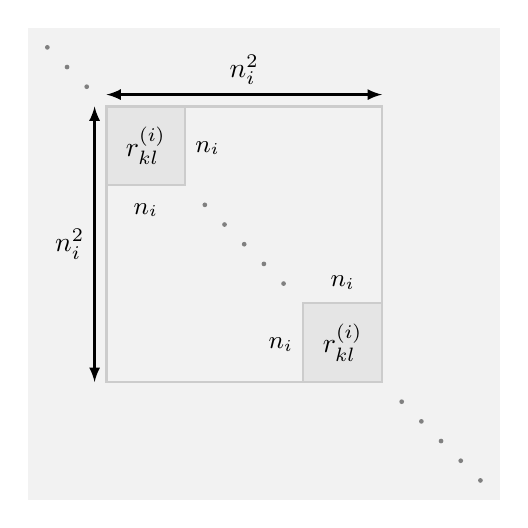
\begin{tikzpicture}[>=latex,thick]
\fill[color=gray!10] (-3,-3) rectangle (3,3);
\fill[color=gray!20] (-2,2) rectangle (-1,1);
\draw[color=gray!40] (-2,2) rectangle (-1,1);
\fill[color=gray!20] (0.5,-0.5) rectangle (1.5,-1.5);
\draw[color=gray!40] (0.5,-0.5) rectangle (1.5,-1.5);
\draw[color=gray!40] (-2,2) rectangle (1.5,-1.5);
\draw[color=gray!40] (-2,2) -- (-1.5,2);
\draw[color=gray!40] (0.5,-0.5) -- (1,-0.5);
\draw[color=gray!40] (0.5,-0.5) -- (0.5,-1);
\foreach \x in {2.75,2.5,2.25,0.75,0.5,0.25,0,-0.25,-1.75,-2,-2.25,-2.5,-2.75}{
	\fill[color=gray] (-\x,\x) circle[radius=0.03];
}
\node at (-1.5,1.5) {$r^{(i)}_{kl}$};
\node at (-1.5,1) [below] {\small $n_i\mathstrut$};
\node at (-1,1.5) [right] {\small $n_i\mathstrut$};
\node at (1,-1) {$r^{(i)}_{kl}$};
\node at (0.5,-1) [left] {\small $n_i\mathstrut$};
\node at (1,-0.5) [above] {\small $n_i\mathstrut$};
\draw[<->] (-2,2.15) -- (1.5,2.15);
\node at (-0.25,2.15) [above] {$n_i^2\mathstrut$};
\draw[<->] (-2.15,2) -- (-2.15,-1.5);
\node at (-2.15,0.25) [left] {$n_i^2\mathstrut$};
\end{tikzpicture}}
\right)
\]
enthält.
Jeder Block besteht aus $n_i$ identischen $n_i\times n_i$ Unterblöcken.
Die Matrixelemente $r^{(i)}_{kl}(g)$ dieser Unterblöcke bilden eine
orthonormierte Basis des Unterraumes der zu $\varrho_i$ isomorphen
Darstellungen in der regulären Darstellung.

\begin{beispiel}
Die zyklische Gruppe $C_n=\{0,\dots,n-1\}$ der Reste modulo $n$ hat $n$
Elemente.
Da sie abelsch ist, sind die irreduziblen Darstellungen eindimensional.
Da die Gruppe von $1$ erzeugt wird, ist die Darstellung $\varrho$ durch
das Element $\varrho(1)$ vollständig festgelegt.
Wegen $\varrho(n)=\varrho(0)=1$ muss $\varrho(n)=\varrho(1)^n =1$ sein,
d.~h.~$\varrho(1)=e^{2\pi ik/n}$ mit $k\in \{0,\dots,n-1\}$.
Die zugehörigen Funktionen auf $C_n$ sind  die Funktionen
$x\mapsto e^{2\pi ikx}$.
Aus der allgemeinen Theorie der Darstellungen folgt jetzt, dass diese
Funktionen bezüglich des Skalarproduktes
\[
\langle f,g\rangle
=
\frac{1}{n} \sum_{x=0}^{n-1} \overline{f(x)} g(x)
\]
orthonormiert sind.
Damit haben wir die Basisfunktionen der diskreten harmonischen
Analysis für die Gruppe $C_n$ aus der Darstellungstheorie wiedergewonnen.
\end{beispiel}

%
% Zerlegung der regulären Darstellung einer kompakten Lie-Gruppe
%
\subsubsection{Zerlegung der regulären Darstellung einer kompakten Lie-Gruppe}
Die Zerlegung der regulären Darstellung funktioniert auch für eine
Lie-Gruppe, was aber etwas aufwendiger zu beweisen ist.
Insbesondere ist es nicht sinnvoll, vom Charakter der regulären Darstellung
zu sprechen, da die reguläre Darstellung eine unendlichdimensionale 
Darstellung ist.
Es gilt aber weiterhin, dass endlichdimensionale irreduzible
Darstellungen genau dann isomorph sind, wenn ihr Skalarprodukt $1$ ist.
Auch die Matrixelemente einer $n$-dimensionalen irreduziblen Darstellungen
sind $n^2$ orthonormierte Funktionen, die eine Basis der $n$ in der
regulären Darstellung von $G$ vorkommenden Kopien der irreduziblen
Darstellung sind.

\begin{beispiel}
Die Gruppe $\mathbb{R}/2\pi\mathbb{Z}$ der Winkel ist abelsch.
Die Matrixelemente sind Funktionen, die unter der Translation invariant
sind, dies sind die Funktionen $x\mapsto e^{ikx}$ mit $k\in \mathbb{Z}$.
Als Skalarprodukt ist
\[
\langle f,g\rangle
=
\frac{1}{2\pi}
\int_0^{2\pi} \overline{f(x)}g(x)\,dx
\]
zu verwenden.
Die allgemeine Theorie zeigt dann, dass die Funktionen $e^{ikx}$ eine
orthonormierte Basis der integrierbaren Funktionen auf der $G$ ist.
Damit haben wir die Theorie der Fourier-Reihen aus der Darstellungstheorie
gewonnen.
\end{beispiel}






